%% HAND-WRITTEN. Reusable placeholder float for a figure that does not exist yet.
%%
%%   \duckplaceholder{<caption text>}{<label>}
%%
%% Draws a large cartoon duck in pure TikZ inside a framed box and captions it
%% "PLACEHOLDER -- <caption text>". Deliberately impossible to miss on a page
%% proof: a figure that is still missing must never look like a figure that is
%% merely small. No external image file and no package beyond tikz (already
%% loaded by pgfplots).
%%
%% \providecommand so that inputting this file twice in one document is safe.

\providecommand{\duckplaceholder}[2]{%
  \begin{figure}[htbp]
    \centering
    \setlength{\fboxrule}{1.2pt}%
    \setlength{\fboxsep}{6pt}%
    \fbox{%
      \begin{minipage}{0.84\linewidth}
        \centering
        {\bfseries\large FIGURE NOT YET DRAWN}\\[2mm]
        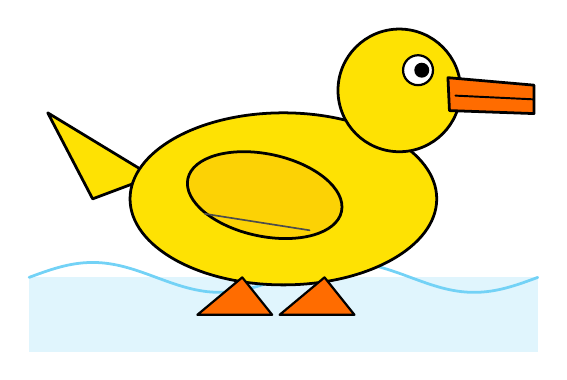
\begin{tikzpicture}[line join=round, line cap=round, scale=0.95]
          % --- water ---------------------------------------------------
          \fill[cyan!12] (-3.4,-2.05) rectangle (3.4,-1.05);
          \draw[cyan!55, line width=1pt]
            (-3.4,-1.05) sin (-2.55,-0.85) cos (-1.7,-1.05)
                         sin (-0.85,-1.25) cos (0,-1.05)
                         sin (0.85,-0.85)  cos (1.7,-1.05)
                         sin (2.55,-1.25)  cos (3.4,-1.05);
          % --- tail ----------------------------------------------------
          \fill[yellow!85!orange, draw=black, line width=1pt]
            (-1.75,0.30) -- (-3.15,1.15) -- (-2.55,0.00) -- cycle;
          % --- neck ----------------------------------------------------
          \draw[yellow!85!orange, line width=0.62cm] (0.70,0.35) -- (1.45,1.30);
          \draw[black, line width=1pt] (0.47,0.50) -- (1.22,1.45);
          \draw[black, line width=1pt] (0.93,0.20) -- (1.68,1.15);
          % --- body ----------------------------------------------------
          \fill[yellow!85!orange, draw=black, line width=1pt]
            (0,0) ellipse [x radius=2.05, y radius=1.15];
          % --- wing ----------------------------------------------------
          \draw[black, line width=1pt, fill=yellow!70!orange, rotate around={-12:(-0.25,0.05)}]
            (-0.25,0.05) ellipse [x radius=1.05, y radius=0.55];
          \draw[black!70, line width=0.6pt] (-1.05,-0.20) -- (0.35,-0.42);
          % --- head ----------------------------------------------------
          \fill[yellow!85!orange, draw=black, line width=1pt]
            (1.55,1.45) circle [radius=0.82];
          % --- beak ----------------------------------------------------
          \fill[orange!85!red, draw=black, line width=1pt]
            (2.20,1.62) -- (3.35,1.52) -- (3.35,1.14) -- (2.22,1.18) -- cycle;
          \draw[black, line width=0.7pt] (2.30,1.38) -- (3.35,1.33);
          % --- eye -----------------------------------------------------
          \fill[white, draw=black, line width=0.8pt] (1.80,1.72) circle [radius=0.20];
          \fill[black] (1.85,1.72) circle [radius=0.10];
          % --- feet ----------------------------------------------------
          \fill[orange!85!red, draw=black, line width=0.8pt]
            (-0.55,-1.05) -- (-1.15,-1.55) -- (-0.15,-1.55) -- cycle;
          \fill[orange!85!red, draw=black, line width=0.8pt]
            (0.55,-1.05) -- (-0.05,-1.55) -- (0.95,-1.55) -- cycle;
        \end{tikzpicture}\\[2mm]
        {\bfseries\large PLACEHOLDER}
      \end{minipage}}
    \caption{PLACEHOLDER -- #1}
    \label{#2}
  \end{figure}}
